\chapter{Datenbank}
\label{cha:Datenbank}


\section{Dokumentation der Datenbank}
\label{sec:DokuDerDatenbank}
Als Datenbank ist f�r ``PrakMan'' die Nutzung unterschiedlicher Angebote m�glich. Unterst�tzt werden derzeit Hypersonic-DB (HSQL, sowohl lokal als auch extern) und PostgreSQL. Daf�r wurde der Aufbau der Tabellen relativ einfach gehalten, um allen Datenbanken gerecht zu werden.\\
In den folgenden Abschnitten wird der genaue Aufbau der f�r ``PrakMan'' ben�tigten Tabellen beschrieben bzw. dargestellt.

\section{Entity- Relationship- Modell (ERM) der Datenbank}
\label{sec:ERM}
Der Aufbau der Datenbank, welche f�r den Praktikums-Manager unabdingbar ist, ist in den Grafiken auf den Seiten \pageref{img:ERM-Tutor-Events}, \pageref{img:ERM-Tutor-Events-Projekt} und \pageref{img:ERM-Tutor-Events-Termine} dargestellt. Einige Tabellen werden dabei mehrfach gezeigt, um jeweils den Zusammenhang zu den Grundobjekten (Student, Tutor, Event) darzustellen.

\begin{figure}[hb]
\begin{center}
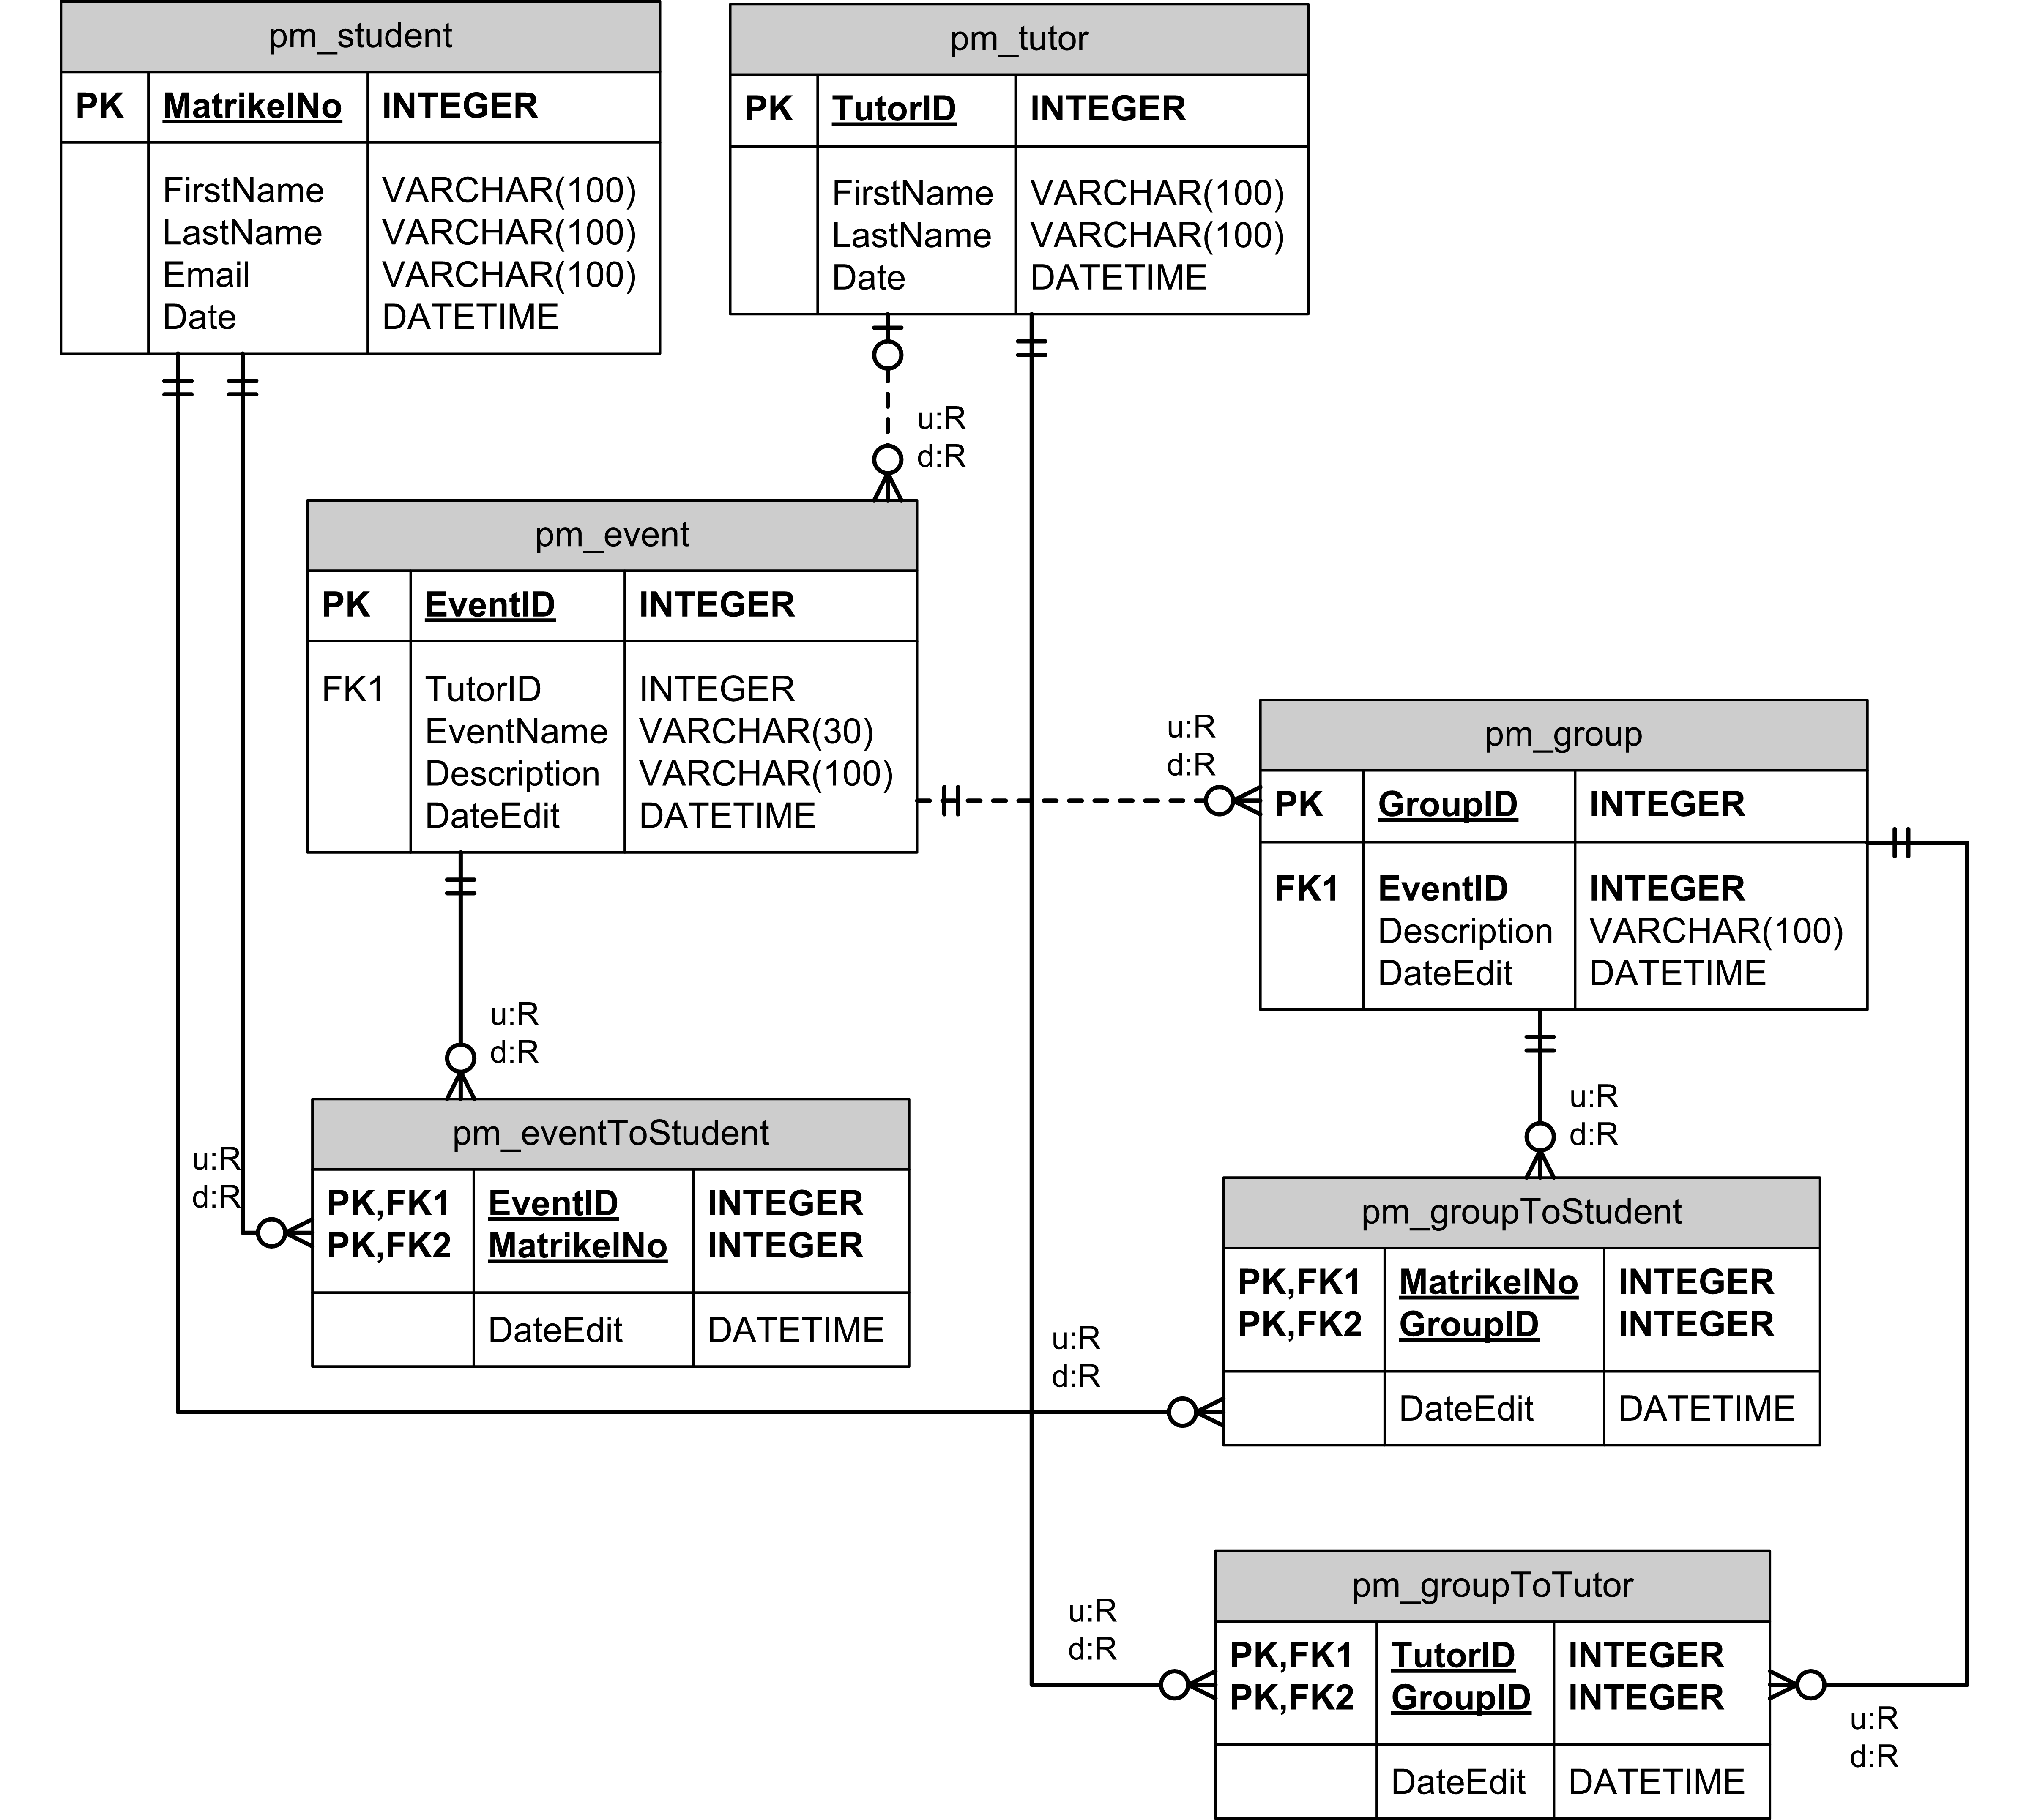
\includegraphics[width=\gfxwidth]{gfx/PrakMan_DB_student_tutor_event}
\caption{ER-Modell der Beziehungen zwischen Student, Tutor und Event}
\label{img:ERM-Tutor-Events}
\end{center}
\end{figure}

\begin{figure}[hb]
\begin{center}
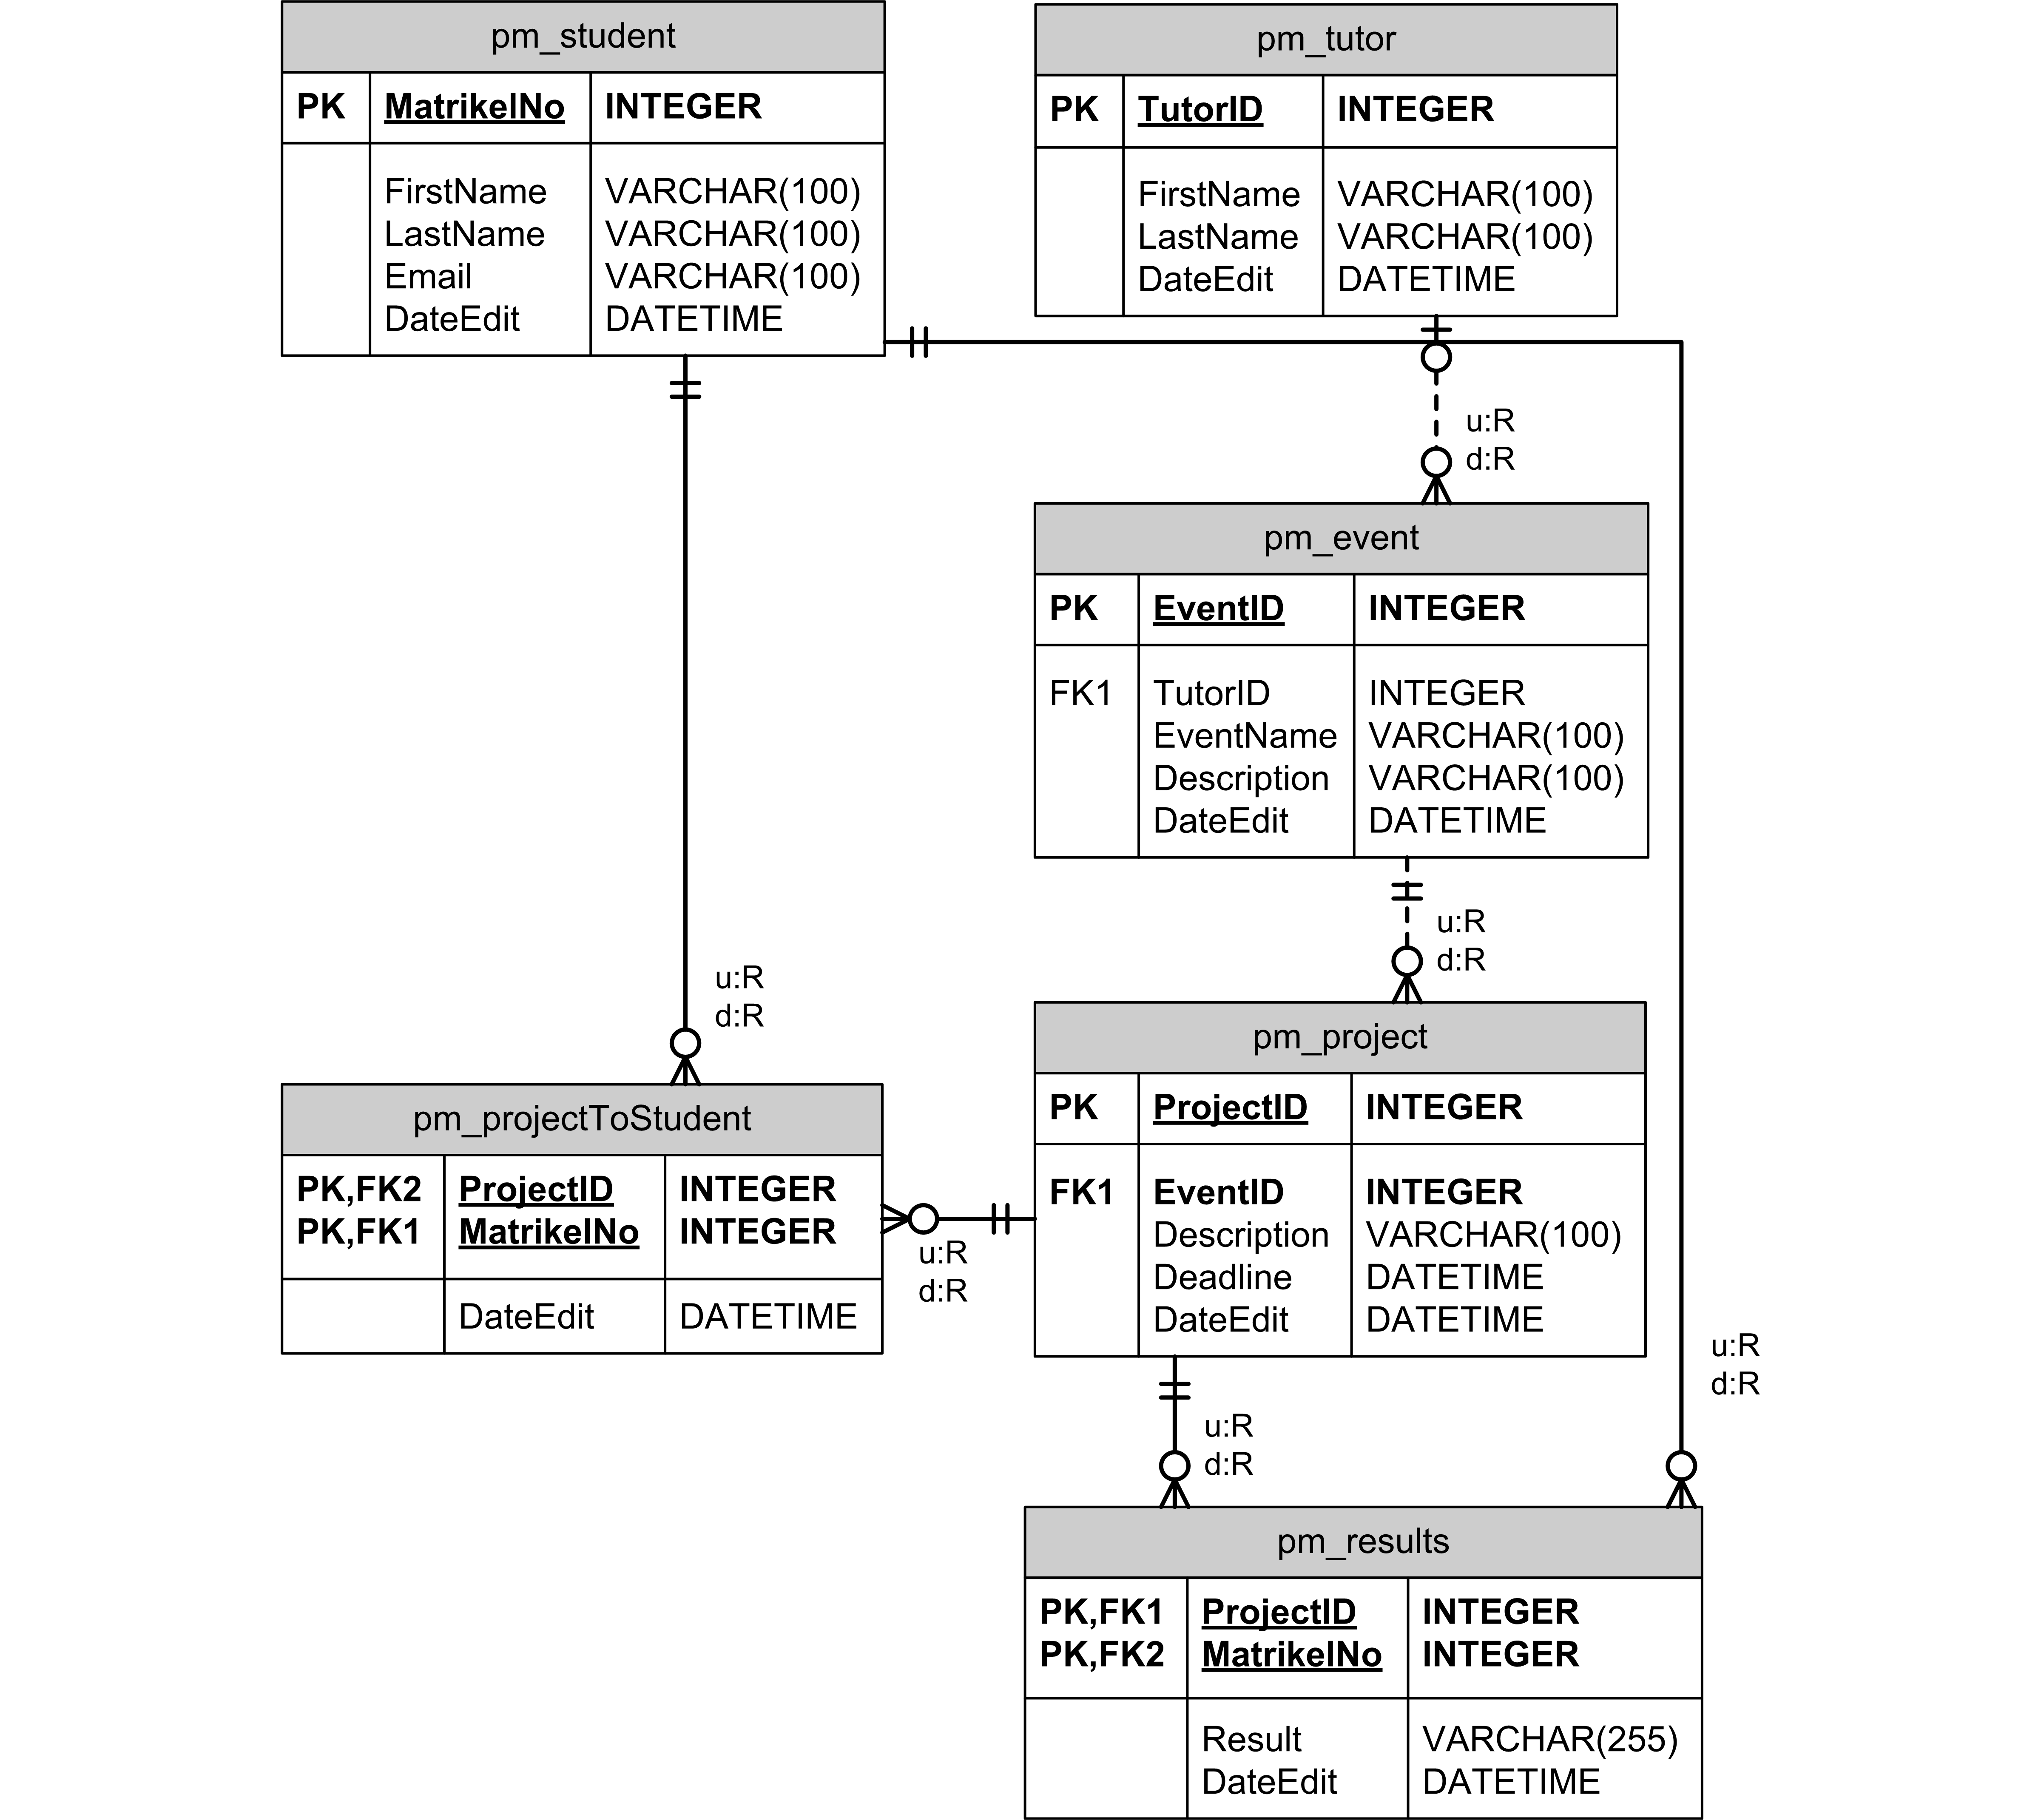
\includegraphics[width=\gfxwidth]{gfx/PrakMan_DB_ERM_event_project}
\caption{ER-Modell der Beziehungen zwischen Student, Tutor, Events und Projekten}
\label{img:ERM-Tutor-Events-Projekt}
\end{center}
\end{figure}

\begin{figure}[hb]
\begin{center}
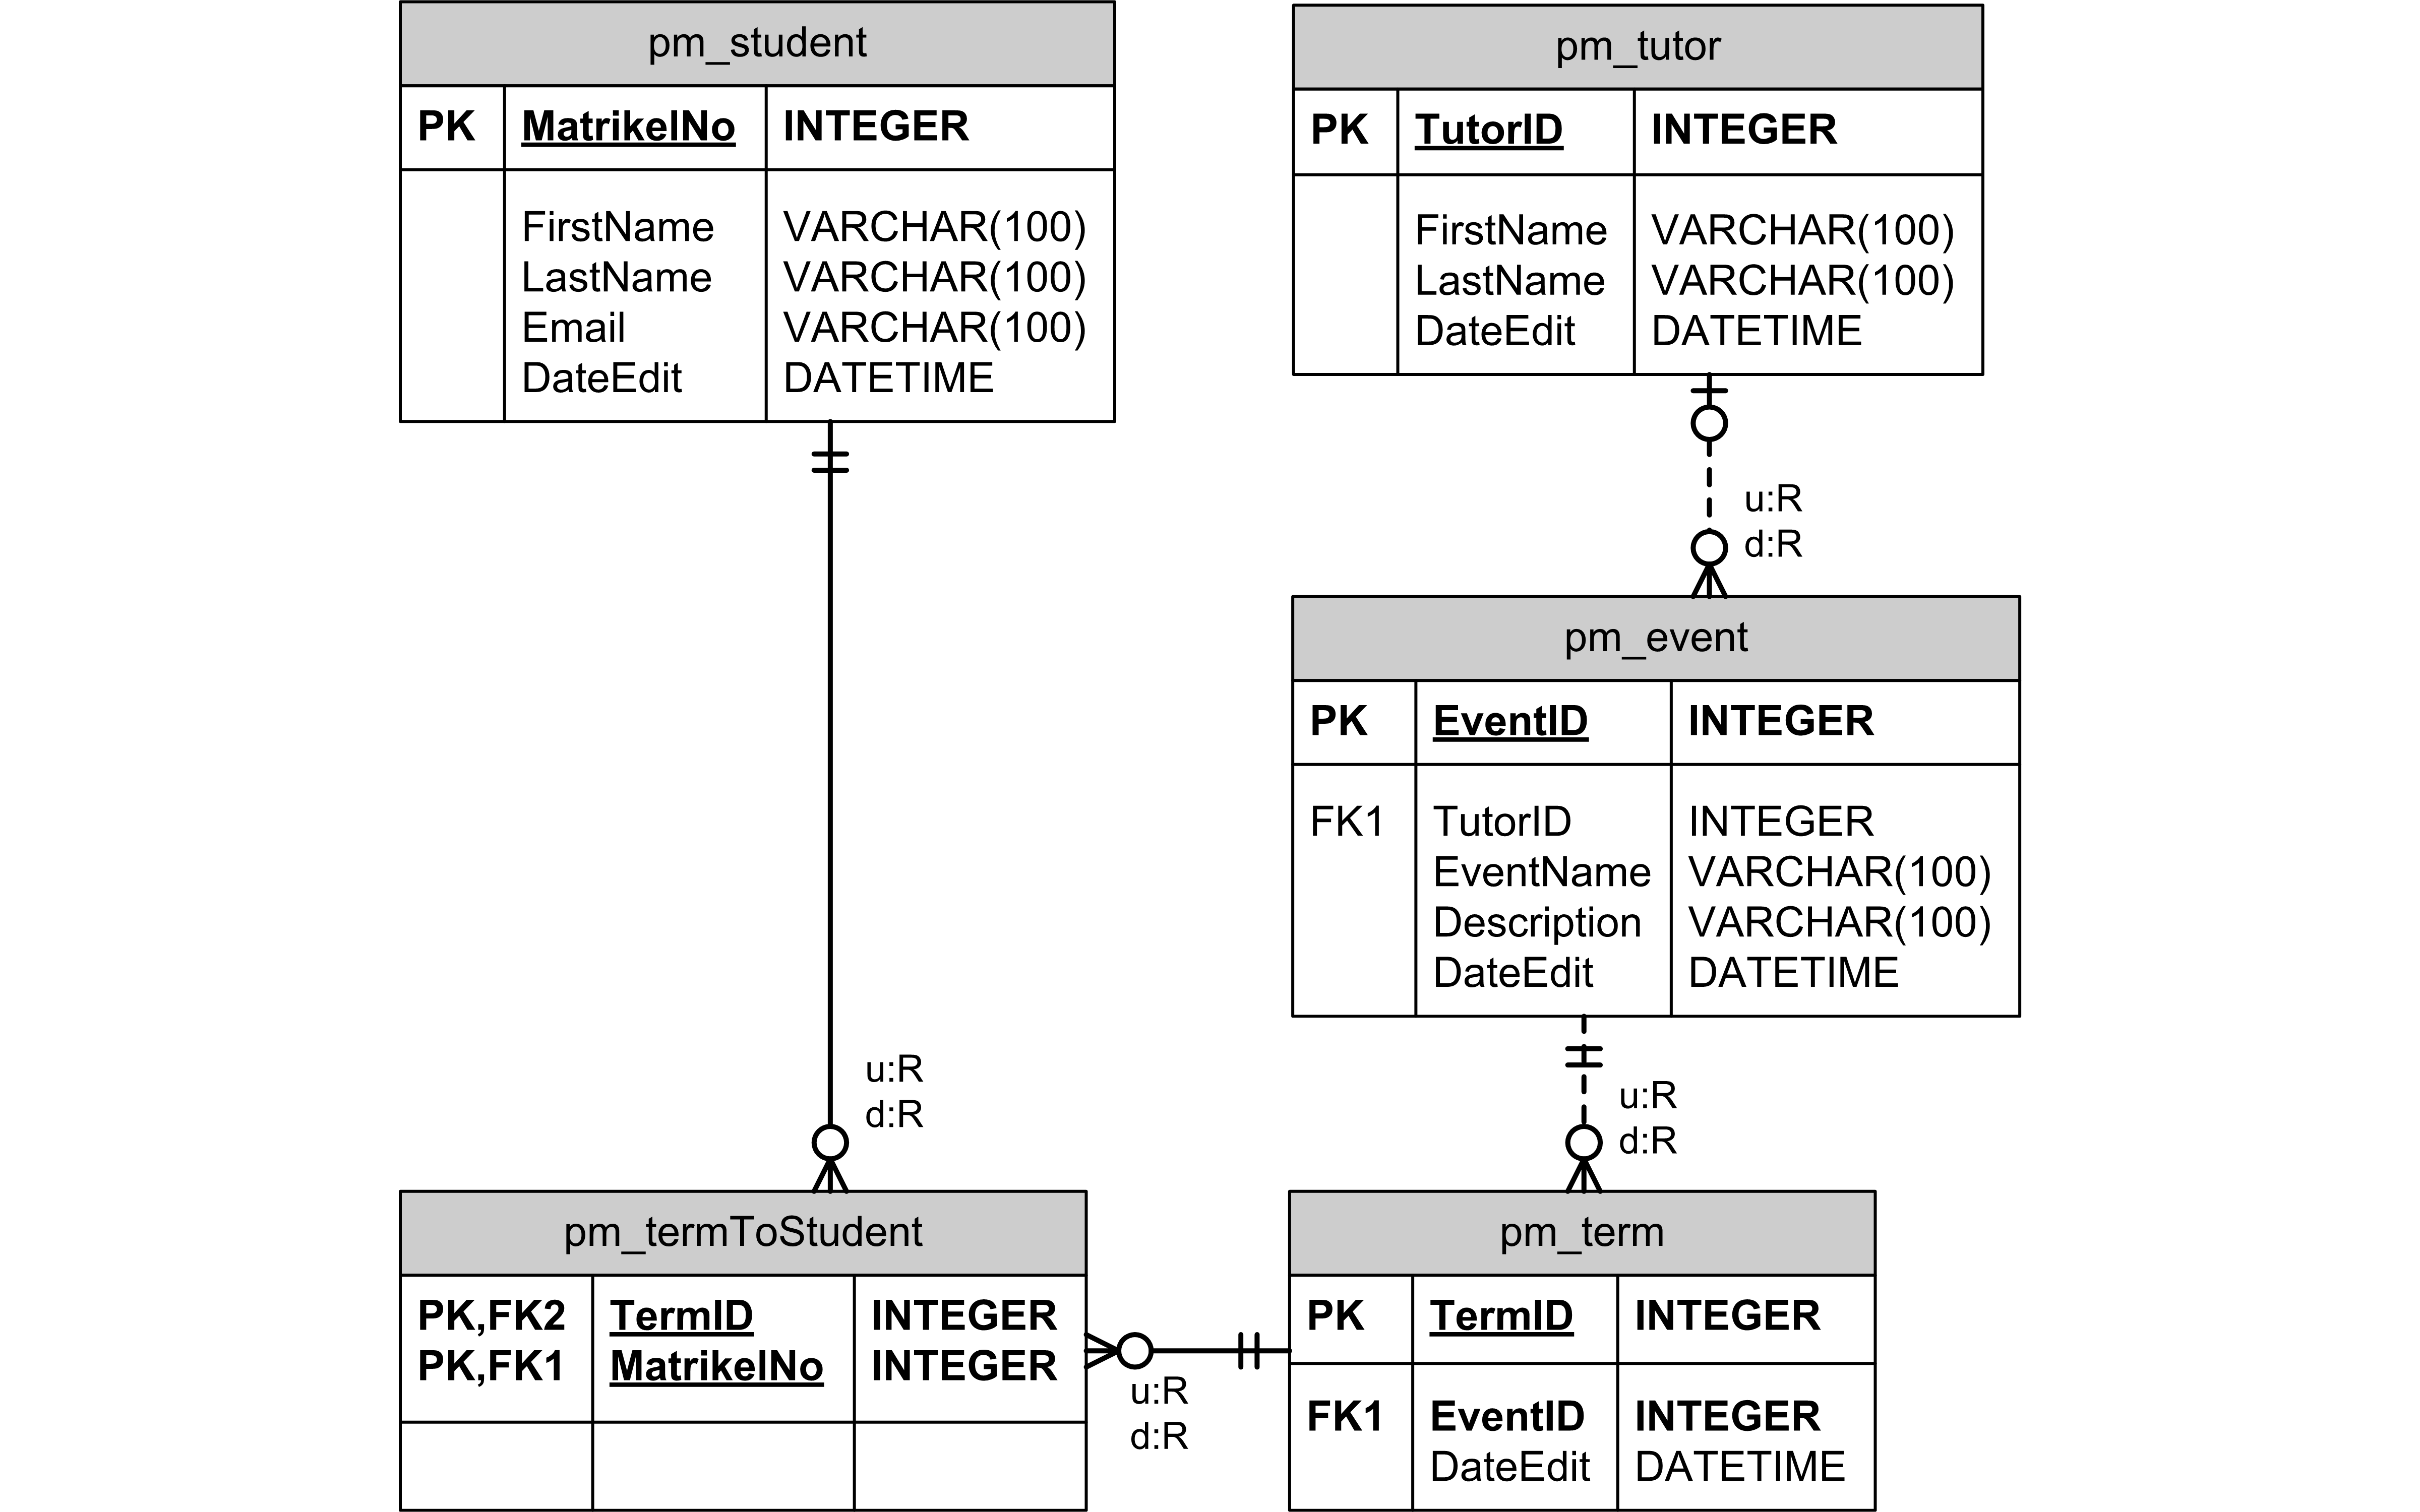
\includegraphics[width=\gfxwidth]{gfx/PrakMan_DB_ERM_terms}
\caption{ER-Modell der Beziehungen zwischen Student, Tutor, Events und Terminen}
\label{img:ERM-Tutor-Events-Termine}
\end{center}
\end{figure}

\section{Pr�fung des Relationenschemas auf Einhaltung der Normalisierung}
\label{sec:PruefungRelationsschema}

\subsection{1te Normalform}
\label{subsec:1teNormalform}
Alle Tabellen enthalten atomare Attribute. Listen werden durch zus�tzliche Tabellen dargestellt.\\
Somit ist 1NF erf�llt.

\subsection{2te Normalform}
\label{subsec:2teNormalform}
Alle Relationen sind in 1NF.
Au�erdem haben alle Objekte (Studenten, Tutoren, Events, Termine, Gruppen, Projekte) eine in der entsprechenden Relation einmalige Identifikationsnummer (ID). Jegliche Verweise laufen ausschlie�lich �ber solche IDs. Somit bestehen auch s�mtliche Prim�rschl�ssel aus einer ID oder mehreren IDs, von denen alle weiteren Attribute voll funktional abh�ngen. Weitere Daten werden f�r Referenzen nicht ben�tigt, weshalb auch keine redundaten Daten in diesem Zusammenhang auftreten k�nnen.\\
Somit ist 2NF erf�llt.

\subsection{3te Normalform}
\label{subsec:3teNormalform}
Alle Relationen sind in 2NF.
Auch hier ist die Eindeutigkeit ausschlie�lich �ber die vorhandenen IDs hergestellt. Keine andere Kombination von Schl�sselkandidaten existiert und w�rde eine weitere Identifikation eines Objekts in einer Tabelle erm�glichen.
Demnach k�nnen auch keine Nicht-Schl�ssel-Attribute von anderen Nicht-Schl�ssel-Attributen funktional abh�ngen.\\
Somit ist 3NF erf�llt.

\section{Funktionsbeschreibung der Formatprogramme}
\label{sec:FunktionsbeschreibungFormatprogramme}

Zum Erstellen der Tabellen wird kein Formatprogramm ben�tigt. Bei Programmstart wird automatisch eine passende SQL-Datei gelesen und die Tabellen, falls n�tig, erstellt.

\section{Funktionsbeschreibung der Reportprogramme}
\label{sec:FunktionsbeschreibungReportprogramme}

Es wurde kein spezielles Reportprogramm zum Auslesen der Datenbank geschrieben, da das, in verbesserter Darstellung, eine Funktion das Programms ``PrakMan'' ist.

\section{Funktionsbeschreibung der SQL- /ESQL- /JDBC- Programme}
\label{sec:FunktionsbeschreibungSQLJDBC}

Wie bereits in Punkt \ref{sec:FunktionsbeschreibungFormatprogramme} erw�hnt, liest ``PrakMan'' zum Erstellen der Tabellen eine SQL-Datei ein und erstellt nach diesen Vorgaben, falls n�tig, das Grundger�st f�r eine korrekte Funktionsweise. Die genannte Datei ist ``CreateTables.sql'', welche sich im Paket prakman.io.sql befindet. Auf diese Weise lassen sich bei �nderung eines Datenbankprogramms auf eine andere Version sehr einfach die Tabellen anpassen.\\
F�r die Zukunft w�re auch eine Erweiterung denkbar, die f�r jede Datenbankform eine extra angepasste SQL-Datei enth�lt, um optimal die M�glichkeiten der unterschiedlichen Datenbanktypen nutzen zu k�nnen.
